\documentclass[conference]{IEEEtran}
\IEEEoverridecommandlockouts
\usepackage{cite}
\usepackage{amsmath,amssymb,amsfonts}
\usepackage{graphicx}
\usepackage{textcomp}
\usepackage{booktabs}
\usepackage{array}
\usepackage{url}
\renewcommand{\ttdefault}{cmtt}

\makeatletter
\providecommand{\linebreakand}{\end{@IEEEauthorhalign}\hfill\mbox{}\par\mbox{}\hfill\begin{@IEEEauthorhalign}}
\makeatother

\begin{document}

\title{How Do Silicon Respondents Use Demographics?\\ Prompting, Fine-Tuning and Held-Out-Item Transfer in India}

\author{
\IEEEauthorblockN{Krishank Ayyella}
\IEEEauthorblockA{Department of Computer Science\\
\textit{[University Name]}\\
{}[City, Country]\\
krishankayyella@{}[domain]}
\and
\IEEEauthorblockN{Bhanuj Bhalla}
\IEEEauthorblockA{Department of Computer Science\\
\textit{[University Name]}\\
{}[City, Country]\\
bhanujbhalla@{}[domain]}
\linebreakand
\IEEEauthorblockN{Yash Bhende}
\IEEEauthorblockA{Department of Computer Science\\
\textit{[University Name]}\\
{}[City, Country]\\
yashbhende@{}[domain]}
\and
\IEEEauthorblockN{Ishaan Bansal}
\IEEEauthorblockA{Department of Computer Science\\
\textit{[University Name]}\\
{}[City, Country]\\
ishaanbansal@{}[domain]}
}

\maketitle

\begin{abstract}
Silicon sampling uses a language model, prompted with a demographic profile, as a stand-in survey respondent. Benchmarks report that such respondents match or trail simple classifiers, but say little about \emph{what the profile contributes} or \emph{what supervised adaptation changes}. We study these questions on Pew Research Center's Religion in India survey ($N{=}29{,}999$) and WVS-7 India ($N{=}1{,}692$), scoring every method on identical respondent--item rows against matched classifiers. On a 200-respondent Pew subset, zero-shot Qwen2.5-7B-Instruct scores <<zs.chat.methods.zs_base_chat.acc|p1>>\% (majority class <<zs.chat.methods.majority.acc|p1>>\%). It uses the profile heavily (the profile explains <<dr.variance_decomposition.zero_shot_soft.incremental_demo|p0>>\% of its prediction variance against <<dr.variance_decomposition.true.incremental_demo|p0>>\% of real answers) but its group differences correlate only $r={<<dr.sub200_zero_shot_soft.r|d2>>}$ with real ones, and the profile lowers accuracy by <<zp.p2_minus_p0|a1>> points relative to no profile. QLoRA fine-tuning on 184{,}853 respondent-level examples reaches <<pe.overall.finetuned.accuracy|p1>>\% on all 6{,}000 held-out respondents (majority <<pe.overall.majority.accuracy|p1>>\%, logistic regression <<pe.overall.logistic.accuracy|p1>>\%, GBM <<pe.overall.gboost.accuracy|p1>>\%), is well calibrated (ECE <<ff.overall.finetuned.ece|d3>>), and on the subset is <<zs.chat.paired.zs_base_chat-finetuned.diff|a1>> points above zero-shot. In a held-out-item test, an approximate re-implementation of the adapter shows no detectable gain over its base on eight unseen questions (<<ae.unseen.methods.adapter_raw.acc|p1>>\% vs.\ <<ae.unseen.methods.base_raw.acc|p1>>\%); the in-domain gain is larger by <<did.did|a1>> points over respondents, but with eight items per side this difference is not distinguishable from zero at the item level. A 120B zero-shot model scores <<api.methods.groq.acc|p1>>\% on <<api.n_resp|int>> respondents, below the majority class (difference not significant). Logistic regression needs about 400 labelled respondents, and gradient boosting about 1{,}600, to clear the majority class. On WVS-7 India three zero-shot LLMs score 22 to 26\% on 15 items where the majority class scores 21 to 25\%, and their group differences carry no directional signal.
\end{abstract}

\begin{IEEEkeywords}
silicon sampling, survey simulation, demographic conditioning, QLoRA, transfer, World Values Survey, Pew Research Center, India
\end{IEEEkeywords}

\section{Introduction}

``Silicon sampling'' conditions a language model on a sociodemographic profile and treats its answer as that person's survey response, a possible low-cost complement to polling \cite{argyle2023}. Reports are mixed: models can reproduce demographic--attitude correlations in US data \cite{argyle2023}, yet show substantial misalignment with many groups \cite{santurkar2023}; at the individual level they match or trail statistical baselines trained on the same demographics \cite{chen2026,miranda2025}, are reported to over-attribute attitudes to demographics and inflate between-group gaps \cite{chen2026}, and persona variables explain little real variance \cite{hu2024}. What these benchmarks do not isolate is the \emph{role of the profile itself}. Does a prompted model use the demographic information in the right direction? What does supervised adaptation on respondent-level data change? And does that adaptation carry over to questions the model was never trained on, the one setting in which a classical model fitted per item has no labels to learn from?

We address these questions for India, using two public surveys and controls that separate the profile's contribution from the model's prior: a no-profile prompt, a label-free prior correction, a same-model fine-tuned comparison, and a held-out-item transfer test.

\textbf{Research questions.}
\begin{itemize}
    \item \textbf{RQ1 (use).} How does a prompted LLM use the demographic profile: how much, and in which direction?
    \item \textbf{RQ2 (adaptation).} What does respondent-level fine-tuning change, relative to the zero-shot model and to matched classifiers?
    \item \textbf{RQ3 (transfer).} Does the adaptation transfer to unseen questions?
    \item \textbf{RQ4 (scale and data).} Do a larger zero-shot model or more labelled respondents change the picture?
\end{itemize}

\textbf{Contributions.}
\begin{enumerate}
    \item A set of \emph{profile-use diagnostics} that separate accuracy from mechanism: profile ablation, demographic variance share, and directional validity of group differences (correlation and slope), alongside a label-free prior-corrected control (Section~IV).
    \item Evidence from India (two surveys; fine-tuning evaluated on 6{,}000 held-out respondents, zero-shot controls on 200) that a zero-shot 7B model uses the profile heavily but with weak direction and no accuracy benefit, and that respondent-level fine-tuning recovers most, though not all, of the accuracy and direction gap to matched classifiers (Section~V-A, V-B).
    \item A held-out-item transfer test in which the fine-tuned adapter shows no detectable accuracy gain on eight unseen questions, reported with its limits: an approximate adapter port, 120 respondents and eight items (Section~V-C).
    \item Checks on scale (a 120B zero-shot model), on how many labelled respondents classical models need, and a WVS-7 replication (Sections~V-D, V-E).
\end{enumerate}

\begin{figure*}[!t]
\centering
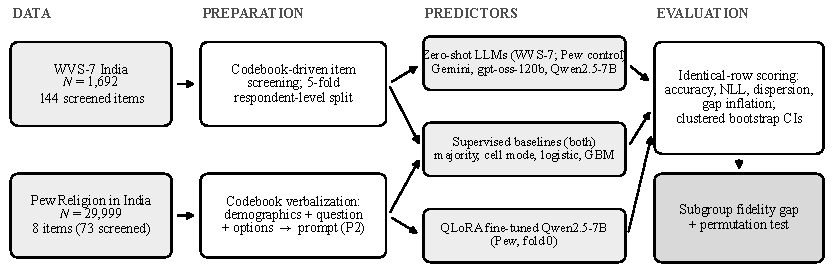
\includegraphics[width=0.98\textwidth]{figs/fig_pipeline.pdf}
\caption{Overview. Both surveys pass through codebook-driven item screening, a respondent-level 5-fold split, and shared verbalization code. Pew supports the profile diagnostics, fine-tuning, and the held-out-item transfer test; WVS-7 supports a zero-shot replication. All scoring is out-of-fold and on identical rows.}
\label{fig:pipeline}
\end{figure*}

\section{Related Work}

\textbf{Simulating respondents.} Argyle et al.~\cite{argyle2023} showed that GPT-3 conditioned on sociodemographic backstories reproduces demographic--attitude correlations in US data (\emph{algorithmic fidelity}). Santurkar et al.~\cite{santurkar2023} found substantial misalignment with many US groups that persists after explicit steering, Durmus et al.~\cite{durmus2023} found cross-national differences in whose opinions models resemble, and Bisbee et al.~\cite{bisbee2024} documented reduced variance and prompt sensitivity. Hu and Collier~\cite{hu2024} show that persona variables explain under 10\% of annotation variance and that persona prompting helps only modestly, most where persona effects are strongest. Shankar et al.~\cite{shankar2026} audit religious viewpoints across Asian populations and find minorities poorly represented.

\textbf{Baselines and over-determination.} Miranda and Balbi~\cite{miranda2025} find individual-level performance comparable between LLMs and random forests on ANES, with the forests often marginally ahead, while LLMs match aggregate distributions better. Chen et al.~\cite{chen2026} evaluate four models, two of them frontier Claude models, on GSS and 63-country WVS against marginal, lookup, logistic and random-forest baselines, and report that no model beats the strongest baseline, that models over-determine attitudes by demographics (a variance-explained ``stereotyping index''), and that segment gaps are inflated two- to fourfold. Ziaei~\cite{ziaei2026} reports loss of response variance after post-training and survey fine-tuning. Two recent reports on other surveys find negligible individual-level recovery: Wang~\cite{wang2026} on the European Social Survey, where a neighbouring-country average beats every model configuration, and Lam et al.~\cite{lam2026} on Singapore, where frontier models give moderately faithful means but understate variance.

\textbf{Adaptation.} Kim and Lee~\cite{kim2023} train respondent-level embeddings over a frozen language model; Suh et al.~\cite{suh2025} and Cao et al.~\cite{cao2025} fine-tune on survey data, the former generalising to unseen subpopulations and surveys, the latter to unseen questions, countries and a new survey but least well to unseen questions; Choi et al.~\cite{choi2026} find that fine-tuning on small pilot samples gives the most balanced structural and marginal fidelity on a Korean survey; Krsteski et al.~\cite{krsteski2025} find rectification more valuable than fine-tuning when human data are scarce; Sun et al.~\cite{sun2024} condition on group-level demographics. Robbani~\cite{robbani2026} finds, for Mistral-7B on US panel data, that demographic information is readable in internal representations but swapping it moves predictions by under 2\% of the error, a representation-level counterpart to the behavioural profile-use results here.

\textbf{Positioning.} The finding that LLMs do not clearly beat matched baselines, and the over-determination and gap-inflation phenomena, are established~\cite{chen2026,miranda2025,hu2024}; we do not claim them as new and use them as a frame. What we add is (a)~an India-specific study with respondent-level fine-tuning at $N\approx$ 30 thousand and a same-model zero-shot control, (b)~diagnostics that separate how much the profile is used from whether it is used in the right direction, and (c)~a held-out-item test at respondent level, which is where adapted LLMs could in principle add value over classifiers.

\section{Data}

\textbf{Pew Religion in India} \cite{pew2021} is a face-to-face survey of 29{,}999 adults fielded between November 2019 and March 2020. Question wording and labels were parsed from the survey's DDI metadata and 73 items passed screening (binary items, demographic columns, items with missingness above 10\%, and near-unanimous items were excluded). The first eight items of the frozen screened list (religious practice and identity, norms on politics and abortion, sex-selective practice, number of children; $K=4$ to 8 options) are used for fine-tuning. Items 9 to 16 (meditation, self-rated health, trust in health advice, what it takes to be ``truly Indian'', television serials, praying) are never used for training and form the transfer set. Respondents are split into five folds stratified by urban/rural $\times$ income band; this paper uses fold~0 (23{,}999 training, 6{,}000 test respondents; 46{,}209 test rows on the trained items). The prompt (P2) carries nine attributes: sex, age band, marital status, education, religion, caste, urban/rural, region, income band.

\textbf{WVS-7 India} (v6.0 \cite{wvs7}; $N=1{,}692$): 373 candidate items were screened against the codebook to 144; zero-shot runs use 15 of them and the 14-attribute P2 prompt.

\section{Methods}

\subsection{Predictors and controls}

\textbf{Matched baselines} are fit per item on training respondents with exactly the prompt's attributes: majority class, logistic regression and histogram GBM \cite{pedregosa2011} (plus a six-attribute cell mode for WVS). All baselines predict the mode, and all are scored on the same rows as the LLMs.

\textbf{Zero-shot Qwen2.5-7B-Instruct} \cite{qwen2025} is run locally for the 200-respondent subset (4-bit MLX \cite{mlx2023}) and, for the full fold, on a Kaggle T4 (NF4, fp16 compute); the next-token distribution over option tokens gives a hard prediction and probabilities. Conditions: \emph{chat} (chat template, the usual zero-shot use), \emph{raw} (bare prompt, the fine-tuning format), \emph{no profile} (P0: identical prompt per item), and \emph{prior-corrected} (probabilities rescaled by the training marginal over the model's own mean prediction, label-free for test rows).

\textbf{Fine-tuned model.} QLoRA \cite{dettmers2023,hu2022} (4-bit NF4, rank 16, $\alpha{=}32$, dropout 0.05, q/k/v/o projections, 10.1M trainable parameters), one epoch over 184{,}853 examples (23{,}999 respondents), effective batch 32, peak learning rate $2\times10^{-4}$, seed 42, causal loss over the full sequence (prompt and answer tokens); 6.6~h on one GPU. Predictions are the argmax of the next-token distribution over the option digits after the training-format prompt (prompt followed by a blank line), scored on a Kaggle T4 in fp16 with the 4-bit NF4 base, which is the readout used for every zero-shot condition. The original run's own greedy decoding of the same adapter, which ended the prompt without the separator, scores <<ff.lab_acc_same_rows|p1>>\% and agrees with this readout on <<ff.agreement_with_lab|p1>>\% of rows; we report both and use the training-format readout as primary. The transfer test of Section~V-C used an MLX re-implementation of the adapter on a 4-bit MLX base, which is approximate.

\textbf{Larger zero-shot model.} gpt-oss-120b \cite{gptoss2025} (Groq free tier, low reasoning effort) on a nested subset of respondents with the same prompts.

\subsection{Diagnostics}

All use normalised answer indices in $[0,1]$ on ordinal items.

\textbf{Demographic variance share.} The increase in $R^2$ when profile dummies are added to item fixed effects, for the predictions and for the true answers (the analogue of the variance-explained index of~\cite{chen2026}).

\textbf{Directional validity.} For each (item, axis, category) cell with at least 15 respondents (100 on the full Pew fold, 8 on WVS-7, where cells are smaller), the group difference is the category mean minus the item mean, for predictions and for truth. We report Pearson $r$ between predicted and true differences and the OLS slope of predicted on true (slope below 1: attenuation; above 1: inflation). Intervals resample respondents; because resampling attenuates cell means they sit below the point estimates and should be read as a measure of uncertainty, not as exact coverage. The variance share uses soft (probability-weighted) predictions for the zero-shot model and hard predictions for the fine-tuned model and GBM.

\textbf{Distributional fidelity.} For each (item, subgroup category) cell with at least 40 respondents, the Jensen--Shannon divergence (base 2) between the mean predicted probability vector and the empirical answer distribution, averaged over cells; this uses probabilities rather than argmax predictions and avoids the inflation of hard predictions. Intervals resample respondents.

\textbf{Accuracy and calibration.} Exact match, MAE on ordinal items and negative log-likelihood (NLL) where probabilities exist; paired respondent-bootstrap differences; Holm correction across axes for subgroup gaps (gap $=$ best minus worst category accuracy, tested by label permutation).

\subsection{Transfer and data-efficiency protocols}

\textbf{Transfer.} The fine-tuned adapter and its base are applied to the eight unseen items for 120 respondents. Labels are used only for scoring; classifiers trained with labels on those items give a ceiling that is unavailable in the new-question setting. The in-domain contrast is computed on the same respondents, and the difference of the two gains is bootstrapped over respondents.

\textbf{Labelled-data requirement.} Classical models are trained on nested respondent subsets ($N=25$ to 23{,}999; five random subsets each) and scored on the same 200 test respondents, giving the number of labelled respondents needed to clear the majority class.

\section{Results}

\subsection{RQ1: the profile is used heavily, not usefully}

\begin{table}[!t]
\caption{Pew, 200 held-out respondents (1{,}548 rows; the direction and variance columns exclude one non-ordinal item, 1{,}351 rows and 182 cells). Dir.\ $r$: correlation between predicted and true group differences. Profile var.: share of variance explained by the profile beyond item effects.}
\label{tab:controls}
\centering
\scriptsize
\setlength{\tabcolsep}{2.6pt}
\begin{tabular}{@{}lrrrr@{}}
\toprule
\textbf{Predictor (200 respondents)} & \textbf{Acc. (\%)} [95\% CI] & \textbf{NLL} & \textbf{Dir. $r$} & \textbf{Profile var.} \\
\midrule
True answers & --- & --- & --- & 4.0\% \\
Majority class (uses labels) & 30.2 [28.1, 32.4] & 1.59 & --- & --- \\
Zero-shot, no profile (P0) & 21.1 [19.1, 23.1] & 3.92 & --- & 0.0\% \\
Zero-shot, profile (chat) & 17.5 [15.7, 19.4] & 3.88 & 0.22 & 29.4\% \\
Zero-shot, prior-corrected & 26.3 [24.0, 28.6] & --- & --- & --- \\
Fine-tuned (lab run, hard) & 37.7 [35.1, 40.3] & --- & 0.58 & 7.1\% \\
Gradient boosting (uses labels) & 40.4 [37.3, 43.4] & 1.43 & 0.64 & 6.1\% \\
\bottomrule
\end{tabular}
\end{table}

Table~\ref{tab:controls} summarises the zero-shot behaviour. With the chat template the model scores <<zs.chat.methods.zs_base_chat.acc|p1>>\% (95\% CI <<zs.chat.methods.zs_base_chat.ci.0|p1>>--<<zs.chat.methods.zs_base_chat.ci.1|p1>>), <<zs.chat.paired.zs_base_chat-majority.diff|a1>> points below the majority class and at chance (<<calc.uniform_pew|p1>>\%); the raw prompt is the same (<<zs.raw.methods.zs_base_raw.acc|p1>>\%, 120 respondents). Removing the profile \emph{raises} accuracy to <<zp.acc_p0|p1>>\%: the profile changes accuracy by <<zp.p2_minus_p0|s1>> points (<<zp.p2_minus_p0_ci.0|s1>> to <<zp.p2_minus_p0_ci.1|s1>>). The model nevertheless reacts strongly to the profile: its prediction changes on <<zp.same_prediction_rate|p0>>\% of rows relative to no profile, and the profile explains <<dr.variance_decomposition.zero_shot_soft.incremental_demo|p0>>\% of its prediction variance, against <<dr.variance_decomposition.true.incremental_demo|p0>>\% for real answers and <<dr.variance_decomposition.gboost.incremental_demo|p0>>\% for GBM. Its group differences are weakly aligned with the truth ($r={<<dr.sub200_zero_shot_soft.r|d2>>}$, 95\% CI <<dr.sub200_zero_shot_soft.r_ci.0|d2>> to <<dr.sub200_zero_shot_soft.r_ci.1|d2>>) and strongly attenuated (slope <<dr.sub200_zero_shot_soft.slope|d2>>). Fig.~\ref{fig:direction} shows the pattern. On the full fold (6{,}000 respondents, 46{,}209 rows) the same model scores <<ff.overall.base_chat.acc|p1>>\% with the chat template (95\% CI <<ff.overall.base_chat.acc_ci.0|p1>>--<<ff.overall.base_chat.acc_ci.1|p1>>) and <<ff.overall.base_raw.acc|p1>>\% with the raw prompt, against <<calc.uniform_pew|p1>>\% for chance and <<ff.overall.majority.acc|p1>>\% for the majority class, so the subset result is not a sampling artefact. A prior correction recovers about two thirds of the distance to the majority class (<<zc.zs_prior_corrected.acc|p1>>\%) but not more, and the model's NLL (<<zs.chat.methods.zs_base_chat.nll|d2>>) is worse than uniform guessing, with probability concentrated on a single option for most respondents (mean top-option share 0.71).

\begin{figure*}[!t]
\centering
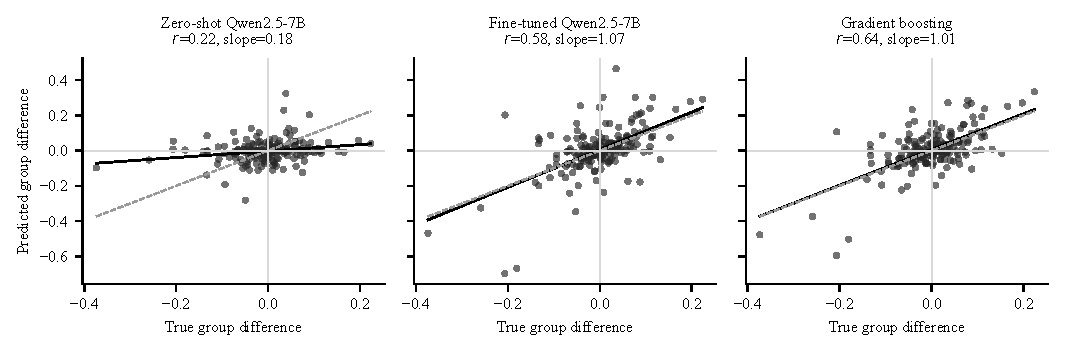
\includegraphics[width=\textwidth]{figs/fig_direction.pdf}
\caption{Predicted versus true group differences for 182 (item, axis, category) cells (200 respondents; item-centred, normalised scale). Dashed: identity. Zero-shot differences are nearly flat and weakly correlated; fine-tuned and GBM predictions track the diagonal.}
\label{fig:direction}
\end{figure*}

On a gender-role subset of WVS-7 the direction is partly right: the zero-shot model predicts the correct sign of the female--male difference on all three gender-role items but inflates its size by 1.1 to 4 times, and on seven of the twelve other items the sign is wrong (exploratory, script wvs\_genderrole.py; 51 to 63 respondents per group, and the true differences on these items are small). We read this as correct direction on a few items where a common stereotype points the same way as the data, not as general use of the profile.

\subsection{RQ2: fine-tuning recovers most of the gap, short of GBM}

\begin{table}[!t]
\caption{Pew fold-0 results, 46{,}209 held-out answers from 6{,}000 respondents. $^\dagger$MAE on ordinal items. $^\S$Error of the predicted subgroup-mean answer on a $[0,1]$ scale (hard predictions).}
\label{tab:pewoverall}
\centering
\footnotesize
\setlength{\tabcolsep}{3pt}
\begin{tabular}{@{}lrrr@{}}
\toprule
\textbf{Method} & \textbf{Accuracy (\%) [95\% CI]} & \textbf{MAE}$^\dagger$ & \textbf{Grp. err.}$^\S$ \\
\midrule
Majority class & 30.4 [29.9, 30.8] & 1.65 & 0.34 \\
Logistic regression & 38.5 [38.0, 39.0] & 1.35 & 0.15 \\
Gradient boosting & 40.0 [39.6, 40.5] & 1.29 & 0.13 \\
Fine-tuned Qwen2.5-7B & 38.0 [37.5, 38.4] & 1.35 & 0.13 \\
\bottomrule
\end{tabular}
\end{table}

On the full fold (Table~\ref{tab:pewoverall}) the fine-tuned model reaches <<pe.overall.finetuned.accuracy|p1>>\% (95\% CI <<pe.overall.finetuned.ci.0|p1>>--<<pe.overall.finetuned.ci.1|p1>>): <<pe.paired.finetuned-majority.diff|s1>> points over the majority class, <<pe.paired.finetuned-logistic.diff|s1>> relative to logistic regression (<<pe.paired.finetuned-logistic.ci.0|s1>> to <<pe.paired.finetuned-logistic.ci.1|s1>>) and <<pe.paired.finetuned-gboost.diff|s1>> relative to GBM, closing <<gc.gap_closed|p0>>\% (<<gc.ci.0|p0>>--<<gc.ci.1|p0>>) of the majority-to-GBM accuracy gap. Its NLL (<<ff.overall.finetuned.nll|d2>>) lies between logistic regression (<<ff.overall.logistic.nll|d2>>) and the majority class (<<ff.overall.majority.nll|d2>>) and above GBM (<<ff.overall.gboost.nll|d2>>), and it is well calibrated (ECE <<ff.overall.finetuned.ece|d3>>). It trails GBM on every item (by 1.2 to 2.7 points); averaging its probabilities with GBM's gives no accuracy gain over GBM ($-$0.2 points, 95\% CI $-$0.5 to $+$0.0). The lab run's decoding gave a constant answer on Q12; under the training-format readout the model predicts the majority answer for most respondents there and its mean probabilities follow the true shares, so that collapse was a property of the decoding, not of the adapter. On the 200-respondent subset it exceeds the zero-shot model by <<zs.chat.paired.zs_base_chat-finetuned.diff|a1>> points (paired 95\% CI <<zs.chat.paired.zs_base_chat-finetuned.ci.1|a1>> to <<zs.chat.paired.zs_base_chat-finetuned.ci.0|a1>>) and beats a prior-corrected zero-shot model by <<zc.paired.finetuned-zs_prior_corrected.diff|a1>> points. Its group differences correlate $r={<<dr.sub200_finetuned.r|d2>>}$ with the truth on the subset (GBM <<dr.sub200_gboost.r|d2>>) and <<dr.full_finetuned.r|d2>> on the full fold (GBM <<dr.full_gboost.r|d2>>), with slope near one on the subset (<<dr.sub200_finetuned.slope|d2>>) and above one on the full fold (<<dr.full_finetuned.slope|d2>>; GBM <<dr.full_gboost.slope|d2>>); the subset and full-fold values use different cell thresholds (15 and 100 respondents) and are not directly comparable. Hard predictions of all three methods inflate between-group differences (<<pd.finetuned.gap_inflation_median|x1>> fine-tuned, <<pd.gboost.gap_inflation_median|x1>> GBM, <<pd.logistic.gap_inflation_median|x1>> logistic), which is consistent with hard argmax predictions inflating group differences in general; we did not test soft predictions for this. Fine-tuned subgroup accuracy gaps differ from zero on five of eight axes after Holm correction (religion 10.0 points, region 8.8, age 2.7, income 1.7, urban/rural 1.3), and differ from GBM's by at most 1.9 points, nominally only for region ($+1.4$, CI 0.1 to 3.5, uncorrected). Scored on probabilities, the fine-tuned model's predicted subgroup distributions are close to the truth: mean Jensen--Shannon divergence <<dist.axes.religion.finetuned.jsd|d3>> across religion cells and <<dist.axes.region.finetuned.jsd|d3>> across region cells, against <<dist.axes.religion.logistic.jsd|d3>> and <<dist.axes.region.logistic.jsd|d3>> for logistic regression, <<dist.axes.religion.majority.jsd|d3>> and <<dist.axes.region.majority.jsd|d3>> for the item marginal, and <<dist.axes.religion.base_raw.jsd|d3>> and <<dist.axes.region.base_raw.jsd|d3>> for the zero-shot model. The fine-tuned model is thus about two to three times further from the truth than the classifiers on religion and region, and more than an order of magnitude closer than the zero-shot model. Tuning the classifiers on a validation split of the training respondents changes little (logistic <<tb.logistic.acc|p1>>\%, GBM <<tb.gboost.acc|p1>>\%), so the gap to GBM is not due to under-tuned classifiers (the fine-tuned configuration itself was not tuned).

\subsection{RQ3: no detectable gain on unseen items}

\begin{figure*}[!t]
\centering
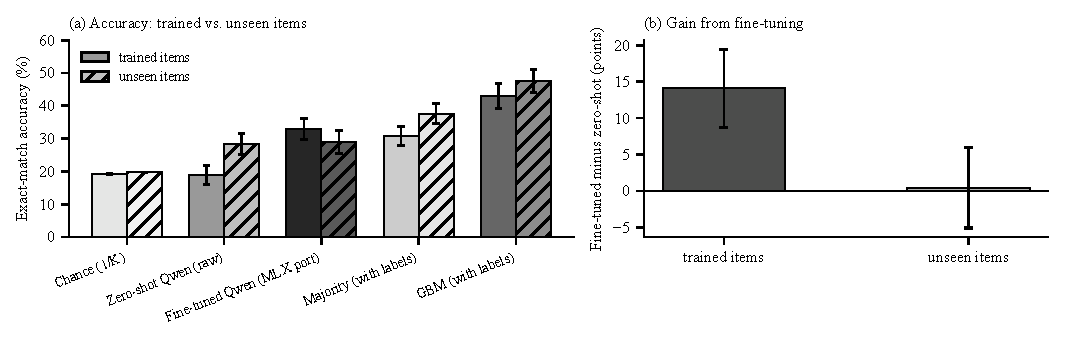
\includegraphics[width=\textwidth]{figs/fig_transfer.pdf}
\caption{(a)~Accuracy on the eight trained and eight unseen items (120 respondents; 95\% respondent-bootstrap CIs). (b)~Gain of the fine-tuned model over its zero-shot base with paired 95\% CIs. Classifiers marked ``with labels'' are not available for a genuinely new question.}
\label{fig:transfer}
\end{figure*}

\begin{table}[!t]
\caption{Transfer to eight unseen Pew items (<<ae.unseen.n_resp|int>> respondents, <<ae.unseen.n_rows|int>> rows). Dir.\ $r$ as in Table~\ref{tab:controls}.}
\label{tab:transfer}
\centering
\scriptsize
\setlength{\tabcolsep}{3pt}
\begin{tabular}{@{}lrrr@{}}
\toprule
\textbf{Method (8 unseen items)} & \textbf{Acc. (\%)} [95\% CI] & \textbf{NLL} & \textbf{Dir. $r$} \\
\midrule
Chance (1/K) & 19.7 [19.7, 19.8] & 1.65 & --- \\
Zero-shot Qwen2.5-7B & 28.5 [25.2, 31.6] & 2.39 & $-$0.02 \\
Fine-tuned Qwen2.5-7B (port) & 28.9 [25.5, 32.4] & 1.69 & 0.24 \\
Majority (uses labels) & 37.6 [34.6, 40.7] & 1.46 & --- \\
Logistic (uses labels) & 44.7 [41.6, 47.8] & 1.34 & 0.79 \\
GBM (uses labels) & 47.6 [44.1, 50.9] & 1.32 & 0.80 \\
\bottomrule
\end{tabular}
\end{table}

The fine-tuned adapter was applied to eight Pew items it never saw. On the trained items the MLX re-implementation scores <<ae.trained.methods.adapter_raw.acc|p1>>\% against <<ae.trained.methods.base_raw.acc|p1>>\% for its base (a gain of <<ae.trained.paired.adapter_raw-base_raw.diff|s1>> points) and <<ae.trained.methods.original_ft.acc|p1>>\% for the original lab-run model, so the port reproduces much of the effect but is weaker, with <<ae.trained.agree_adapter_raw_original_ft|p0>>\% row agreement and a similar directional validity (<<ae.trained.direction.adapter_raw.r|d2>> against <<ae.trained.direction.original_ft.r|d2>> for the original). On the unseen items (Table~\ref{tab:transfer}, Fig.~\ref{fig:transfer}) the adapter scores <<ae.unseen.methods.adapter_raw.acc|p1>>\% and its base <<ae.unseen.methods.base_raw.acc|p1>>\%, a difference of <<ae.unseen.paired.adapter_raw-base_raw.diff|s1>> points (<<ae.unseen.paired.adapter_raw-base_raw.ci.0|s1>> to <<ae.unseen.paired.adapter_raw-base_raw.ci.1|s1>>), against <<did.gain_trained|s1>> in domain: over respondents the in-domain gain exceeds the unseen gain by <<did.did|a1>> points (95\% CI <<did.did_ci.0|a1>>--<<did.did_ci.1|a1>>). That interval treats the eight items on each side as fixed. Across items the difference is 14.0 points with a standard error of 10.2 (permutation $p=0.18$), and the unseen gain ranges from $-21$ to $+36$ points per item, so we do not claim that the in-domain gain is reliably larger than the unseen gain; the safe reading is that no gain on unseen items is detectable. Two weaker signals remain: calibration (NLL <<ae.unseen.methods.base_raw.nll|d2>> to <<ae.unseen.methods.adapter_raw.nll|d2>>, still above the uniform value of 1.65) and the direction of group differences ($r={<<ae.unseen.direction.adapter_raw.r|d2>>}$, 95\% CI <<ae.unseen.direction.adapter_raw.r_ci.0|d2>> to <<ae.unseen.direction.adapter_raw.r_ci.1|d2>>, against $<<ae.unseen.direction.base_raw.r|d2>>$ for the base). Classifiers fitted with labels on these items reach <<ae.unseen.methods.majority.acc|p1>>\% (majority), <<ae.unseen.methods.logistic.acc|p1>>\% and <<ae.unseen.methods.gboost.acc|p1>>\%, so in this setting the adapted LLM does not offer a usable substitute for new-question data. The test uses the approximate port, 120 respondents and eight items, and a single narrow training set; it does not show that broader fine-tuning would also fail to transfer.

\subsection{RQ4: scale and data}

\textbf{Larger zero-shot model.} gpt-oss-120b on <<api.n_resp|int>> respondents (<<api.n_rows|int>> rows) scores <<api.methods.groq.acc|p1>>\% (<<api.methods.groq.ci.0|p1>>--<<api.methods.groq.ci.1|p1>>): <<api.paired.groq-majority.diff|a1>> points below the majority class (<<api.methods.majority.acc|p1>>\%, difference not significant), against <<api.qwen_zs_on_same_rows|p1>>\% for the 7B model on the same rows, and <<api.paired.groq-ft.diff|a1>> points below the fine-tuned 7B model (<<api.paired.groq-ft.ci.1|a1>> to <<api.paired.groq-ft.ci.0|a1>>). This is a different, larger model and we did not vary scale within a family, so we cannot attribute the difference from the 7B model to scale; it is at the majority class, not beyond.

\textbf{Labelled data.} Classical models need substantial labelled data to beat the majority class. Averaged over five random subsets, logistic regression is at the majority level for $N\le100$ respondents (<<lcb.100.logistic.acc_mean_over_subsets|p1>>\% against <<lcb.100.majority.acc_mean_over_subsets|p1>>\% at $N=100$), exceeds it by <<calc.lc_gap400|s1>> points at $N=400$ (<<lcb.400.logistic.acc_mean_over_subsets|p1>>\%) and by <<calc.lc_gap1600|s1>> at $N=1{,}600$ (<<lcb.1600.logistic.acc_mean_over_subsets|p1>>\%); GBM clears the majority class in accuracy only at about 1{,}600 respondents (<<lcb.1600.gboost.acc_mean_over_subsets|p1>>\%) and still has worse NLL than the majority class there (<<lcb.1600.gboost.nll_mean_over_subsets|d2>> against <<lcb.1600.majority.nll_mean_over_subsets|d2>>). On the same 200 test respondents, the fine-tuned 7B model (trained on 23{,}999 respondents) scores <<zs.chat.methods.finetuned.acc|p1>>\%, below logistic regression trained on 1{,}600 respondents (<<lcb.1600.logistic.acc_mean_over_subsets|p1>>\%). Whether LLM adaptation is more sample-efficient than classical models in this low-data regime is the open question most likely to favour LLMs; we could not test it reliably with 7B models on available hardware, and a small-model (0.5B) attempt trained on up to 100 respondents collapsed to a near-constant answer, so we draw no conclusion from it.

\begin{figure}[!t]
\centering
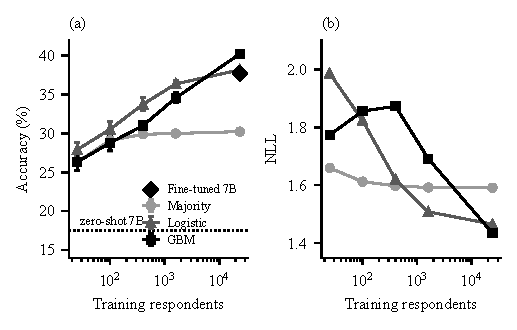
\includegraphics[width=\columnwidth]{figs/fig_lc_classical.pdf}
\caption{Classical models on nested respondent subsets (200 test respondents; mean and SD over five random subsets). (a)~Accuracy; the 7B fine-tuned point uses all 23{,}999 training respondents. (b)~NLL (the zero-shot 7B model, 3.88, is off the scale shown).}
\label{fig:lc}
\end{figure}

\subsection{WVS-7 India replication}

Across the 144 screened items the majority class reaches <<w144.majority|p1>>\% and the cell mode <<w144.cell_mode|p1>>\%, against 46.9\% (logistic) and 50.1\% (GBM): demographics add only +1.4 and +4.6 points. On the 15 evaluated items, Gemini 3.1 Flash Lite (30 respondents) scores <<wm.Gemini.llm.acc|p1>>\% and gpt-oss-120b (40) <<wm.gpt-oss.llm.acc|p1>>\%, both within sampling error of the majority class and <<wm.Gemini.gbm_matched.llm_minus|a1>> and <<wm.gpt-oss.gbm_matched.llm_minus|a1>> points below GBM. Zero-shot Qwen2.5-7B (<<wq.n_resp|int>> respondents, <<wq.n_rows|int>> rows) scores <<wq.llm.acc|p1>>\%, <<wq.majority.llm_minus|a1>> points below the majority class (95\% CI <<wq.majority.llm_minus_ci.0|s1>> to <<wq.majority.llm_minus_ci.1|s1>>) and <<wq.gbm_matched.llm_minus|a1>> below GBM. Its group differences show no directional validity ($r={<<wd.qwen_soft.r|d2>>}$, 345 cells; GBM <<wd.gbm.r|d2>>), the profile changes accuracy by <<wd.p0.p2_minus_p0|s1>> points (<<wd.p0.p2_minus_p0_ci.0|s1>> to <<wd.p0.p2_minus_p0_ci.1|s1>>), and on seven of 15 items (nine at a 90\% threshold) it gives the same answer to nearly every respondent. The 15 items are inherited from an earlier run and their majority class is 21 to 25\%, well below the 144-item figure, so LLM scores are compared with the majority class on the same rows. Subgroup gaps are not distinguishable from random group assignment in any of 12 API-model tests (11 of 12 $p>0.05$, none after Holm correction) nor in the 120-respondent run (smallest $p=0.082$); detection thresholds range from 4.5 to 26.7 points, above most gaps seen on Pew (1 to 2.5 points).

\section{Discussion}

\textbf{What the profile does.} A zero-shot model does not ignore the profile; it varies with it far more than real answers do, but in directions that agree with the data only weakly, and the net effect on exact-match accuracy is slightly negative. This is consistent with persona effects being small and noisy~\cite{hu2024} and with over-determination~\cite{chen2026}, We did not vary prompts, so we cannot say whether richer or better-worded demographics would help.

\textbf{What fine-tuning does.} Respondent-level fine-tuning yields item marginals and group differences approaching, but not reaching, a classifier's: accuracy ends <<pe.paired.finetuned-gboost.diff|a1>> points below GBM and <<pe.paired.finetuned-logistic.diff|a1>> below logistic regression, directional validity on the full fold is <<dr.full_finetuned.r|d2>> against <<dr.full_gboost.r|d2>>, and the two models agree on 72\% of predictions. That no gain is detectable on unseen items is compatible with an item-specific mapping from profile to answer; the port, the number of items and the narrow training set mean it is not evidence that no transfer is possible.

\textbf{Where LLM respondents could add value.} Not, on this evidence, as substitutes for labelled data for the same question (matched classifiers are cheaper and more accurate), nor, at 7B with narrow fine-tuning, as predictors for new questions (no accuracy transfer). Remaining candidate settings are those our design cannot test: richer text-conditioned personas, much broader fine-tuning across many items, and aggregate distribution estimation using probabilities rather than argmax.

\textbf{Evaluation practice.} Accuracy comparisons need a majority-class baseline (45.5\% over the 144 WVS-India items); inflation and concentration of hard predictions must be read against baselines that also show them; and subgroup-gap claims need a permutation null and detection thresholds, which at tens of respondents exceed any plausible effect.

\section{Limitations}

\begin{itemize}
    \item \textbf{Single run.} One fold, one seed, one epoch. Scoring used fp16 on a T4 whereas training used bf16, and the lab run's own greedy decoding gives a lower accuracy for the same adapter (<<ff.lab_acc_same_rows|p1>>\%), so results depend on the readout; we use the one that matches training and the zero-shot conditions.
    \item \textbf{Narrow adaptation.} Fine-tuning used eight religion- and fertility-related items on one fold, one seed, one epoch and a full-sequence loss. Transfer to broader item sets, or after training on many items, is untested; the unseen-item null may reflect narrow training.
    \item \textbf{Approximate port.} Transfer and probability results use an MLX re-implementation of the adapter that is about 7 to 8 points weaker than the original adapter scored on CUDA on the same rows, so the transfer comparison is conservative for the original model.
    \item \textbf{Subsets and sample-efficiency.} Controls use nested random subsets (100 to 200 respondents). LLM sample-efficiency was not established: our small-model attempt collapsed (see above).
    \item \textbf{Models.} Zero-shot results cover one 7B model locally and two free-tier API models; we did not test frontier models on these surveys (Chen et al.~\cite{chen2026} did, on US and cross-national data, with the same failures).
    \item \textbf{Items and surveys.} Two surveys, two sets of eight and 15 items; no language axis (WVS interview language is constant). Pew survey weights are not used, so statements are about the sample, not the population.
    \item \textbf{Transfer evidence.} The unseen-item comparison rests on eight items, 120 respondents and an approximate port; item-level uncertainty is large (Section~V-C).
    \item \textbf{Metric.} Exact match on ordinal items with argmax predictions; distributional and aggregate fidelity are not evaluated, and directional-validity cells share respondents across axes.
    \item \textbf{Interpretation.} The variance share is an in-sample $R^2$ increment; accuracy gaps conflate predictability with bias.
\end{itemize}

\textbf{Ethical considerations.} Both datasets are public and de-identified; WVS microdata are not redistributed. Simulated respondents should not replace sampling of real people, especially for groups where fidelity was lower.

\section{Conclusion}

A prompted 7B model varies strongly with a demographic profile but uses it weakly and slightly harmfully; respondent-level fine-tuning recovers most, though not all, of the accuracy and direction gap to classifiers on the trained questions, and shows no detectable accuracy gain on eight new ones. In the settings we tested, matched classifiers remain the benchmark that LLM respondents must beat, and held-out questions at larger scale are the experiment most likely to change that conclusion. Code, scripts (including runners that scale every experiment to a GPU) and raw model outputs accompany this paper.

\section*{Data and Code Availability}
Code and prompts: \url{https://github.com/bhanujjj/silicon-sampling-capstone} (branches \texttt{lab-package}, \texttt{pew-dataset-training}); analysis scripts, local MLX and CUDA runners and raw outputs are distributed with this paper's source. WVS-7 must be obtained from the WVS Association; Pew data are available from Pew Research Center.

\section*{Acknowledgment}
The authors thank their university's AI Lab for GPU access.

\begin{thebibliography}{99}

\bibitem{argyle2023}
L.~P. Argyle, E.~C. Busby, N.~Fulda, J.~R. Gubler, C.~Rytting, and D.~Wingate, ``Out of one, many: Using language models to simulate human samples,'' \emph{Political Analysis}, vol.~31, no.~3, pp. 337--351, 2023.

\bibitem{santurkar2023}
S.~Santurkar, E.~Durmus, F.~Ladhak, C.~Lee, P.~Liang, and T.~Hashimoto, ``Whose opinions do language models reflect?'' in \emph{Proc. ICML}, 2023.

\bibitem{chen2026}
Z.~Chen, D.~Zhu, and L.~N. Zheng, ``When synthetic users fail: A cross-domain benchmark of LLM-simulated human survey responses,'' arXiv:2607.26348, 2026.

\bibitem{miranda2025}
F.~Miranda and P.~P. Balbi, ``Simulating public opinion: Comparing distributional and individual-level predictions from LLMs and random forests,'' \emph{Entropy}, vol.~27, no.~9, Art.~923, Sep. 2025.

\bibitem{hu2024}
T.~Hu and N.~Collier, ``Quantifying the persona effect in LLM simulations,'' in \emph{Proc. 62nd Annu. Meeting Assoc. Comput. Linguistics (ACL)}, vol.~1, Bangkok, Thailand, Aug. 2024, pp. 10289--10307.

\bibitem{durmus2023}
E.~Durmus \emph{et al.}, ``Towards measuring the representation of subjective global opinions in language models,'' arXiv:2306.16388, 2023.

\bibitem{bisbee2024}
J.~Bisbee, J.~D. Clinton, C.~Dorff, B.~Kenkel, and J.~M. Larson, ``Synthetic replacements for human survey data? The perils of large language models,'' \emph{Political Analysis}, vol.~32, no.~4, pp. 401--416, 2024.

\bibitem{shankar2026}
H.~Shankar, V.~S.~P., S.~Margapuri, D.~Mazumder, P.~Kumaraguru, and A.~Chakraborty, ``Mind the gap: Pitfalls of LLM alignment with Asian public opinion,'' in \emph{Proc. Int. AAAI Conf. Web and Social Media (ICWSM)}, 2026, arXiv:2603.06264.

\bibitem{ziaei2026}
R.~Ziaei, ``The limits of simulated societies: How post-training and survey fine-tuning erase cross-cultural variance,'' arXiv:2609.25760, 2026.

\bibitem{kim2023}
J.~Kim and B.~Lee, ``AI-augmented surveys: Leveraging large language models and surveys for opinion prediction,'' arXiv:2305.09620, 2023.

\bibitem{suh2025}
J.~Suh, E.~Jahanparast, S.~Moon, M.~Kang, and S.~Chang, ``Language model fine-tuning on scaled survey data for predicting distributions of public opinions,'' in \emph{Proc. 63rd Annu. Meeting Assoc. Comput. Linguistics (ACL)}, vol.~1, 2025, pp. 21147--21170.

\bibitem{cao2025}
Y.~Cao, H.~Liu, A.~Arora, I.~Augenstein, P.~R\"{o}ttger, and D.~Hershcovich, ``Specializing large language models to simulate survey response distributions for global populations,'' in \emph{Proc. NAACL}, 2025.

\bibitem{krsteski2025}
S.~Krsteski, G.~Russo, S.~Chang, R.~West, and K.~Gligori\'{c}, ``Valid survey simulations with limited human data: The roles of prompting, fine-tuning, and rectification,'' arXiv:2510.11408, 2025.

\bibitem{sun2024}
S.~Sun \emph{et al.}, ``Random silicon sampling: Simulating human sub-population opinion using a large language model based on group-level demographic information,'' arXiv:2402.18144, 2024.

\bibitem{pew2021}
Pew Research Center, ``Religion in India: Tolerance and segregation,'' Jun. 2021.

\bibitem{wvs7}
C.~Haerpfer, R.~Inglehart, A.~Moreno, C.~Welzel, K.~Kizilova, J.~Diez-Medrano, M.~Lagos, P.~Norris, E.~Ponarin, and B.~Puranen (eds.), \emph{World Values Survey: Round Seven, Country-Pooled Datafile Version 6.0.0}. Madrid, Spain and Vienna, Austria: JD Systems Institute \& WVSA Secretariat, 2024, doi:10.14281/18241.24.

\bibitem{pedregosa2011}
F.~Pedregosa \emph{et al.}, ``Scikit-learn: Machine learning in Python,'' \emph{J. Mach. Learn. Res.}, vol.~12, pp. 2825--2830, 2011.

\bibitem{qwen2025}
Qwen Team, ``Qwen2.5 technical report,'' arXiv:2412.15115, 2024.

\bibitem{mlx2023}
A.~Hannun, J.~Digani, A.~Katharopoulos, and R.~Collobert, ``MLX: Efficient and flexible machine learning on Apple silicon,'' software, 2023. [Online]. Available: https://github.com/ml-explore/mlx

\bibitem{dettmers2023}
T.~Dettmers, A.~Pagnoni, A.~Holtzman, and L.~Zettlemoyer, ``QLoRA: Efficient finetuning of quantized LLMs,'' in \emph{Advances in Neural Information Processing Systems (NeurIPS)}, vol.~36, 2023.

\bibitem{hu2022}
E.~J. Hu \emph{et al.}, ``LoRA: Low-rank adaptation of large language models,'' in \emph{Proc. ICLR}, 2022.

\bibitem{gptoss2025}
OpenAI, ``gpt-oss-120b \& gpt-oss-20b model card,'' arXiv:2508.10925, Aug. 2025.

\bibitem{choi2026}
E.~C. Choi, Y.~Kim, P.~Pugalenthi, H.-E. Chen, and B.-R. Huang, ``Beyond the mean: Three-axis fidelity for aligning LLM-based survey simulators from small pilot data,'' in \emph{Pluralistic Alignment Workshop at ICML}, 2026, arXiv:2606.28963.

\bibitem{robbani2026}
F.~D. Robbani, ``Readable, faithful, used: Three dissociable properties of demographic identity in a language model,'' arXiv:2608.18768, 2026.

\bibitem{wang2026}
C.~Wang, ``Silicon sampling answers with country-level assumptions, not individual attitudes: Cross-national evidence from the European Social Survey,'' arXiv:2609.16395, 2026.

\bibitem{lam2026}
N.~H.~Y. Lam, J.~X. Voo, and X.~Ma, ``The conditional superiority of fast silicon sampling,'' arXiv:2608.14079, 2026.

\end{thebibliography}

\end{document}
